%%%%%%%%%%%%%%%%%%%%%%%%%%%%%%%%%%%%%%%%%%%%%%%%%%%%%%%%%%%%%%%%%%%%%%%%%%%%%%%%
\section{Considerações iniciais}

Sistemas de reconhecimento de imagens comumente utilizam uma imagem em níveis de cinza (8-bits -- 256 intensidades) para as etapas subsequentes à extração de características. Dá-se o nome de quantização à etapa responsável por esta redução no nível de cores em uma imagem. Ao aplicar a quantização na etapa de pré-processamento, é esperada a redução da complexidade do vetor de características logo no início do processo, beneficiando todos os passos subsequentes.

Com o objetivo de analisar o impacto do uso da quantização, foram utilizados diferentes parâmetros de quantização, combinados com quatro métodos de extração de cor e um de textura. Esses métodos foram escolhidos de acordo com os resultados apresentados por \citeonline{Penatti2012}, com exceção dos métodos HOG e LBP, também descritores frequentemente utilizados na literatura \cite{Wang2009a}.

Este capítulo descorre sobre a quantização das imagens antes da extração de características, assim como os métodos utilizados, apresentados na Seção~\ref{sec:quantizacao}.

%%%%%%%%%%%%%%%%%%%%%%%%%%%%%%%%%%%%%%%%%%%%%%%%%%%%%%%%%%%%%%%%%%%%%%%%%%%%%%%%
\section{Quantização de imagens}

O pipeline de reconhecimento de imagens comumente envolve um passo de conversão de imagens coloridas em imagens com apenas um canal. Obtem-se, assim, uma imagem quantizada, que pode ser então processada por métodos de extração de características. Dessa forma, cada imagem -- originalmente no espaço de cor RGB -- é convertida a um único canal com $C$ níveis de intensidade. Após, são utilizados os métodos apresentados na Seção \ref{sec:extracao} para extrair as características.
A Figura \ref{fig:quant:quantizationFlow} ilustra esses passos, desde a aquisição até a classificação das imagens.

\begin{figure}[!htbp]
  \begin{center}
    \centering
    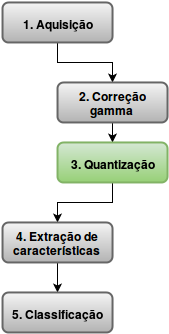
\includegraphics[width=0.25\linewidth]{\detokenize{figuras/quantizacao/quantizationFlow.png}}
  \end{center}
  \caption[O pipeline de reconhecimento de imagens pode envolver uma etapa de conversão de imagens coloridas em imagens em escala de cinza, obtendo uma imagem quantizada que pode ser então processada por métodos de extração de características. O vetor com essas características é então dado como entrada a algum método de classificação.]{O pipeline de reconhecimento de imagens pode envolver uma etapa de converter imagens coloridas em imagens em escala de cinza, obtendo uma imagem quantizada que pode ser então processada por métodos de extração de características. O vetor com essas características é então dado como entrada a um método posterior de classificação, por exemplo a classificação. \textit{Fonte:~Elaborado pela autora.}}
  \label{fig:quant:quantizationFlow}
\end{figure}

Cada método de quantização se comporta diferentemente para uma dada imagem RGB. Por exemplo, o método \emph{Intensidade} mapeia todas as permutações dos mesmos valores em RGB para a mesma cor. Dessa forma, produz um plano no espaço RGB conforme mostrado na Figura \ref{fig:quant:plano}. O efeito do método \emph{Gleam} é similar, mas dada a natureza da função \textit{gamma} (transformação não linear que define a relação entre o valor do pixel e sua real luminância), cobre uma superfície curva. Tal resultado também é alcançado utilizando o método \emph{Intensidade'}. Independente do método utilizado, o resultado é o mapeamento de características cromáticas bem diferentes em valores de intensidades similares. Ou seja, cores distintas podem ser convertidas as cores próximas, podendo aumentar a confusão entre objetos. Os métodos \emph{Luminância} e \emph{Luma} procuram aprimorar a quantização ao ponderar a combinação linear dos canais. Esses métodos são normalmente considerados melhores por se aproximarem ao modelo visual humano, que pondera as cores através do número de cones sensíveis as cores vermelho, verde e azul. O método \emph{MSB} também tenta enfatizar as diferenças cromáticas ao ordenar os bits de cores em um único canal. Para mais detalhes sobre tais métodos, consulte Seção \ref{sec:quantizacao}.

\begin{figure}[!htbp]
  \begin{center}
    \centering
    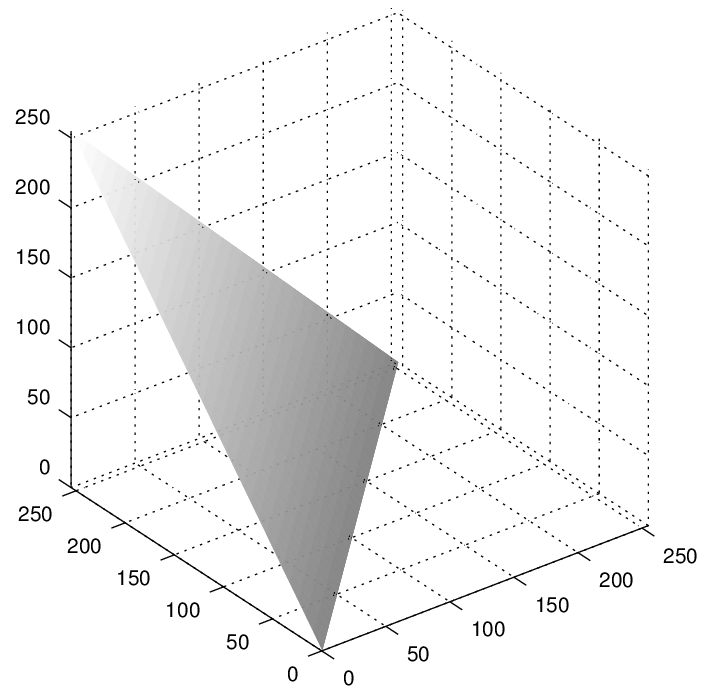
\includegraphics[width=0.5\linewidth]{\detokenize{figuras/quantizacao/plano.png}}
  \end{center}
  \caption[Plano no espaço RGB, computado pelo método de conversão para escala de cinza \emph{Intensidade}, quando um dos canais de cor (vermelho, verde ou azul) possui valor 255. Isso porque este método mapeia todas as permutações dos mesmos valores em RGB para a mesma cor.]{Plano no espaço RGB, computado pelo método de conversão para escala de cinza \emph{Intensidade}, quando um dos canais de cor (vermelho, verde ou azul) possui valor 255. Isso porque este método mapeia todas as permutações dos mesmos valores em RGB para a mesma cor. \textit{Fonte:~\cite{Ponti2016}.}}
  \label{fig:quant:plano}
\end{figure}

Exemplos de imagens obtidas após os métodos de quantização apresentados anteriormente podem ser vistos na Figura \ref{fig:quant:quantizacoes}. A barra de gradientes abaixo da imagem dos pincéis demonstra como os métodos de quantização se comportam dada a variação da cor. É possível notar que os métodos \emph{Luminância} e \emph{MSB} conseguiram melhor discriminar as cores. Além disso, o mapa de cores \emph{MSB} obteve um maior número de cores únicas, quando comparado aos demais métodos.

\begin{figure}[!htbp]
  \begin{center}
    \subfloat[Original]{
      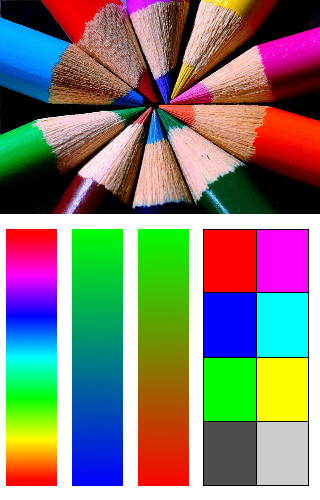
\includegraphics[width=.18\linewidth]{\detokenize{figuras/quantizacao/fig_quanttest.png}}
      \label{fig:quant:original}
    }
    \subfloat[Gleam]{
      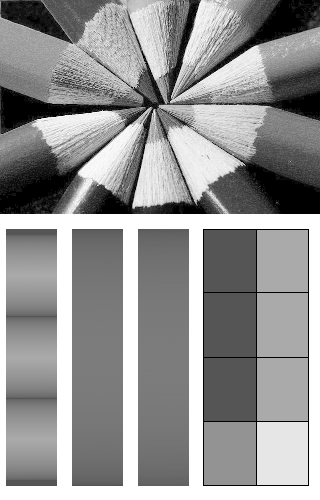
\includegraphics[width=.18\linewidth]{\detokenize{figuras/quantizacao/fig_quantGleam.png}}
    }
    \subfloat[Intensidade]{
      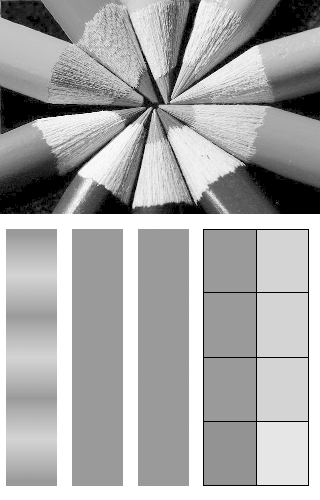
\includegraphics[width=.18\linewidth]{\detokenize{figuras/quantizacao/fig_quantIntensity.png}}
    }
    \subfloat[Luminance]{
      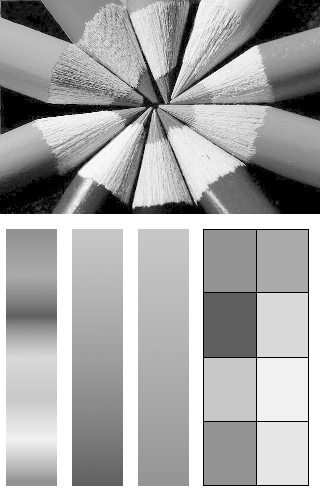
\includegraphics[width=.18\linewidth]{\detokenize{figuras/quantizacao/fig_quantLuminance.png}}
    }
    \subfloat[MSB]{
      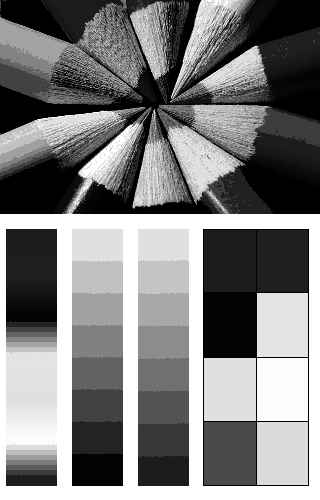
\includegraphics[width=.18\linewidth]{\detokenize{figuras/quantizacao/fig_quantMSB.png}}
    }
    \hspace{0.1\textwidth}
  \end{center}
  \caption[Resultado da aplicação de métodos de quantização. A imagem original \protect\subref{fig:quant:original} resultou em versões de um canal de cor com 232 cores únicas para o método (e) MSB e 184 cores para os demais métodos. Ao analisar-se as barras de gradiente, assim como as paletas de cores, observa-se que os métodos \emph{Luminância} e \emph{MSB} conseguiram uma melhor discriminação entre cores.]{Resultado da aplicação de métodos de quantização. A imagem original \protect\subref{fig:quant:original} resultou em versões de um canal de cor com 232 cores únicas para o método (e) MSB e 184 cores para os demais métodos. Ao analisar-se as barras de gradiente, assim como as paletas de cores, observa-se que os métodos \emph{Luminância} e \emph{MSB} conseguiram uma melhor discriminação entre cores. \textit{Fonte:~\cite{Ponti2016}.}}
  \label{fig:quant:quantizacoes}
\end{figure}

% A Tabela \ref{tab:quantizacao} apresenta alguns exemplos numéricos, com a saída de cada método. Nesse caso, as entradas são tuplas de valores $(R, G, B)$. Note que a correção \textit{gamma} deve ser computada em um intervalo de valores reais $0-1$, que depois é mapeado para o intervalo $0-255$.

Complementando, a Figura \ref{fig:quant:avioes} apresenta mais um exemplo de redução de cores utilizando o método \emph{MSB} para um par de imagens da base de dados \emph{Caltech-101}\footnote{Disponível em \url{http://www.vision.caltech.edu/ImageDatasets/Caltech101/}}. É possível notar que há uma certa preservação das cores, especialmente quando utilizados entre 64 e 256 níveis. Com apenas 32 cores, as imagens ainda lembram a sua versão original, mas há perda considerável de informação, principalmente em regiões da imagem com pouco contraste.

\begin{figure}[!htbp]
  \begin{center}
    \centering
    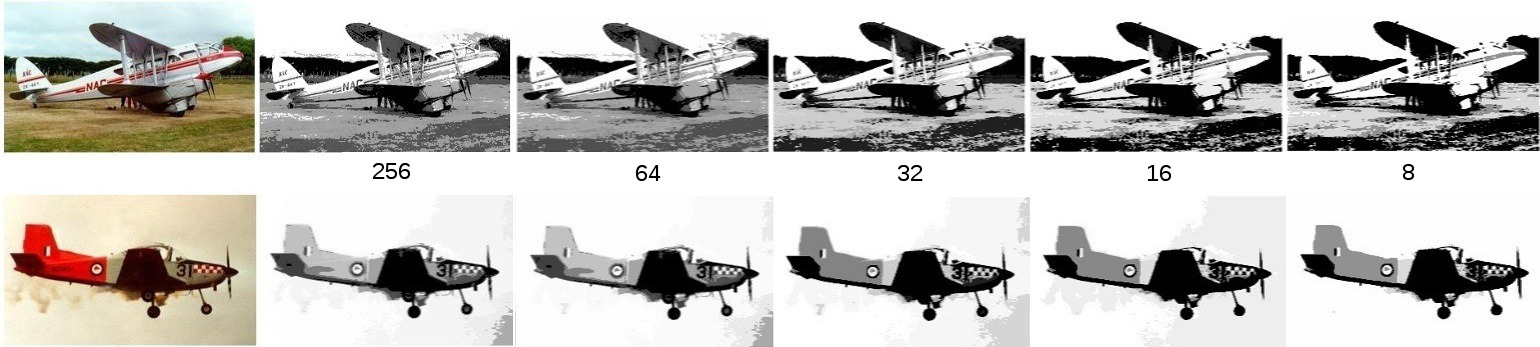
\includegraphics[width=\linewidth]{\detokenize{figuras/quantizacao/fig_quantizationexample.jpg}}
  \end{center}
  \caption[Duas imagens da base de dados \emph{Caltech101} com variações no parâmetro de cor utilizando o método \emph{MSB}. Da esquerda para a direita: imagem original 24-bits e suas versões quantizadas com: 256, 64, 32, 16 e 8 cores.]{Duas imagens da base de dados \emph{Caltech101} com variações no parâmetro de cor utilizando o método \emph{MSB}. Da esquerda para a direita: imagem original 24-bits e suas versões quantizadas com: 256, 64, 32, 16 e 8 cores. \textit{Fonte:~\cite{Ponti2016}.}}
  \label{fig:quant:avioes}
\end{figure}

%%%%%%%%%%%%%%%%%%%%%%%%%%%%%%%%%%%%%%%%%%%%%%%%%%%%%%%%%%%%%%%%%%%%%%%%%%%%%%%%
\section{Considerações finais}


Ao aplicar a quantização na etapa de pré-processamento é esperado a redução da dimensionalidade do vetor de características no início do sistema, beneficiando todas as etapas posteriores. A hipótese é que utilizar um número reduzido de cores vai reduzir significativamente a dimensionalidade, enquanto melhora ou mantém a classificação do sistema.

Espera-se, também, que o método MSB para a quantização tenha uma performance melhor, dada a preservação das cores observada na Figura \ref{fig:quant:avioes}. Os resultados da utilização dos métodos descritos neste capítulo estão no Capítulo \ref{cap:resultados-quantizacao}.
